\section{Basic Game Elements/Mechanics}
Game Mechanics function as basic systems of a game that governs their respective game elements (\cite{adams2012game}). All possible basic functions(represented by algorithms and data structures) and rules in the game are part of the mechanics. The section will discuss about planned game mechanics and their implementation.

\subsection{Web application}
The game will be a web application, this is because web applications are easily accessible and can be played on any device with a web browser. The game will be built using Angular, a popular web application framework. As central storing technique, MongoDB was used. This is because MongoDB is a NoSQL database, which is a good choice for storing JSON data. This database stores all relevant information regarding the
game content and the analytics


\subsection{Level selection}
The game will have multiple levels, each level will have a different set of challenges. The player will have to complete each level to progress to the next. The levels will be designed to increase in difficulty as the player progresses. The levels will be designed to teach the player different concepts of Python programming. The player will have to complete each level to progress to the next. The levels will be designed to increase in difficulty as the player progresses. The levels will be designed to teach the player different concepts of Python programming. The player will have to complete each level to progress to the next. The levels will be designed to increase in difficulty as the player progresses. The levels will be designed to teach the player different concepts of Python programming.





\subsection{Code Input}
The whole user flow of the educational game, game flow\cite{kramarzewski2018practical}, can be simplified. It starts out with the user input, which would be the code submitted, the process would be the gameplay mechanics and the output would be the reward for the player. 

This whole user experience starts with the user input, the submission of code can be done with a simple basic text box.
\begin{figure}[h]
    \centering
    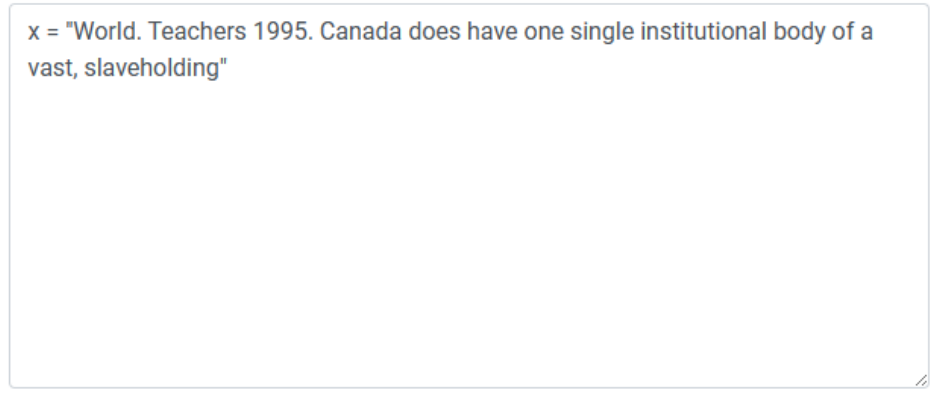
\includegraphics[width=0.5\linewidth]{images/textbox.png}
    \caption{Simple basic text box}
\end{figure}
\\\\
To improve on this submission of code, we can use a code editor like professional integrated development environments (IDEs). An in-browser code editor such as Monaco or ace editor would suffice; additional improvements to build upon a code editor with other options such as night/day mode, a language server to verify Python syntax formatting, and other such Python language features as it is not natively implemented within editors such as Monaco. Other features that should be implemented to help with user experience would be code completion, syntax/semantic highlighter, definition provider, formatting provider, and more.
\begin{figure}[H]
    \centering
    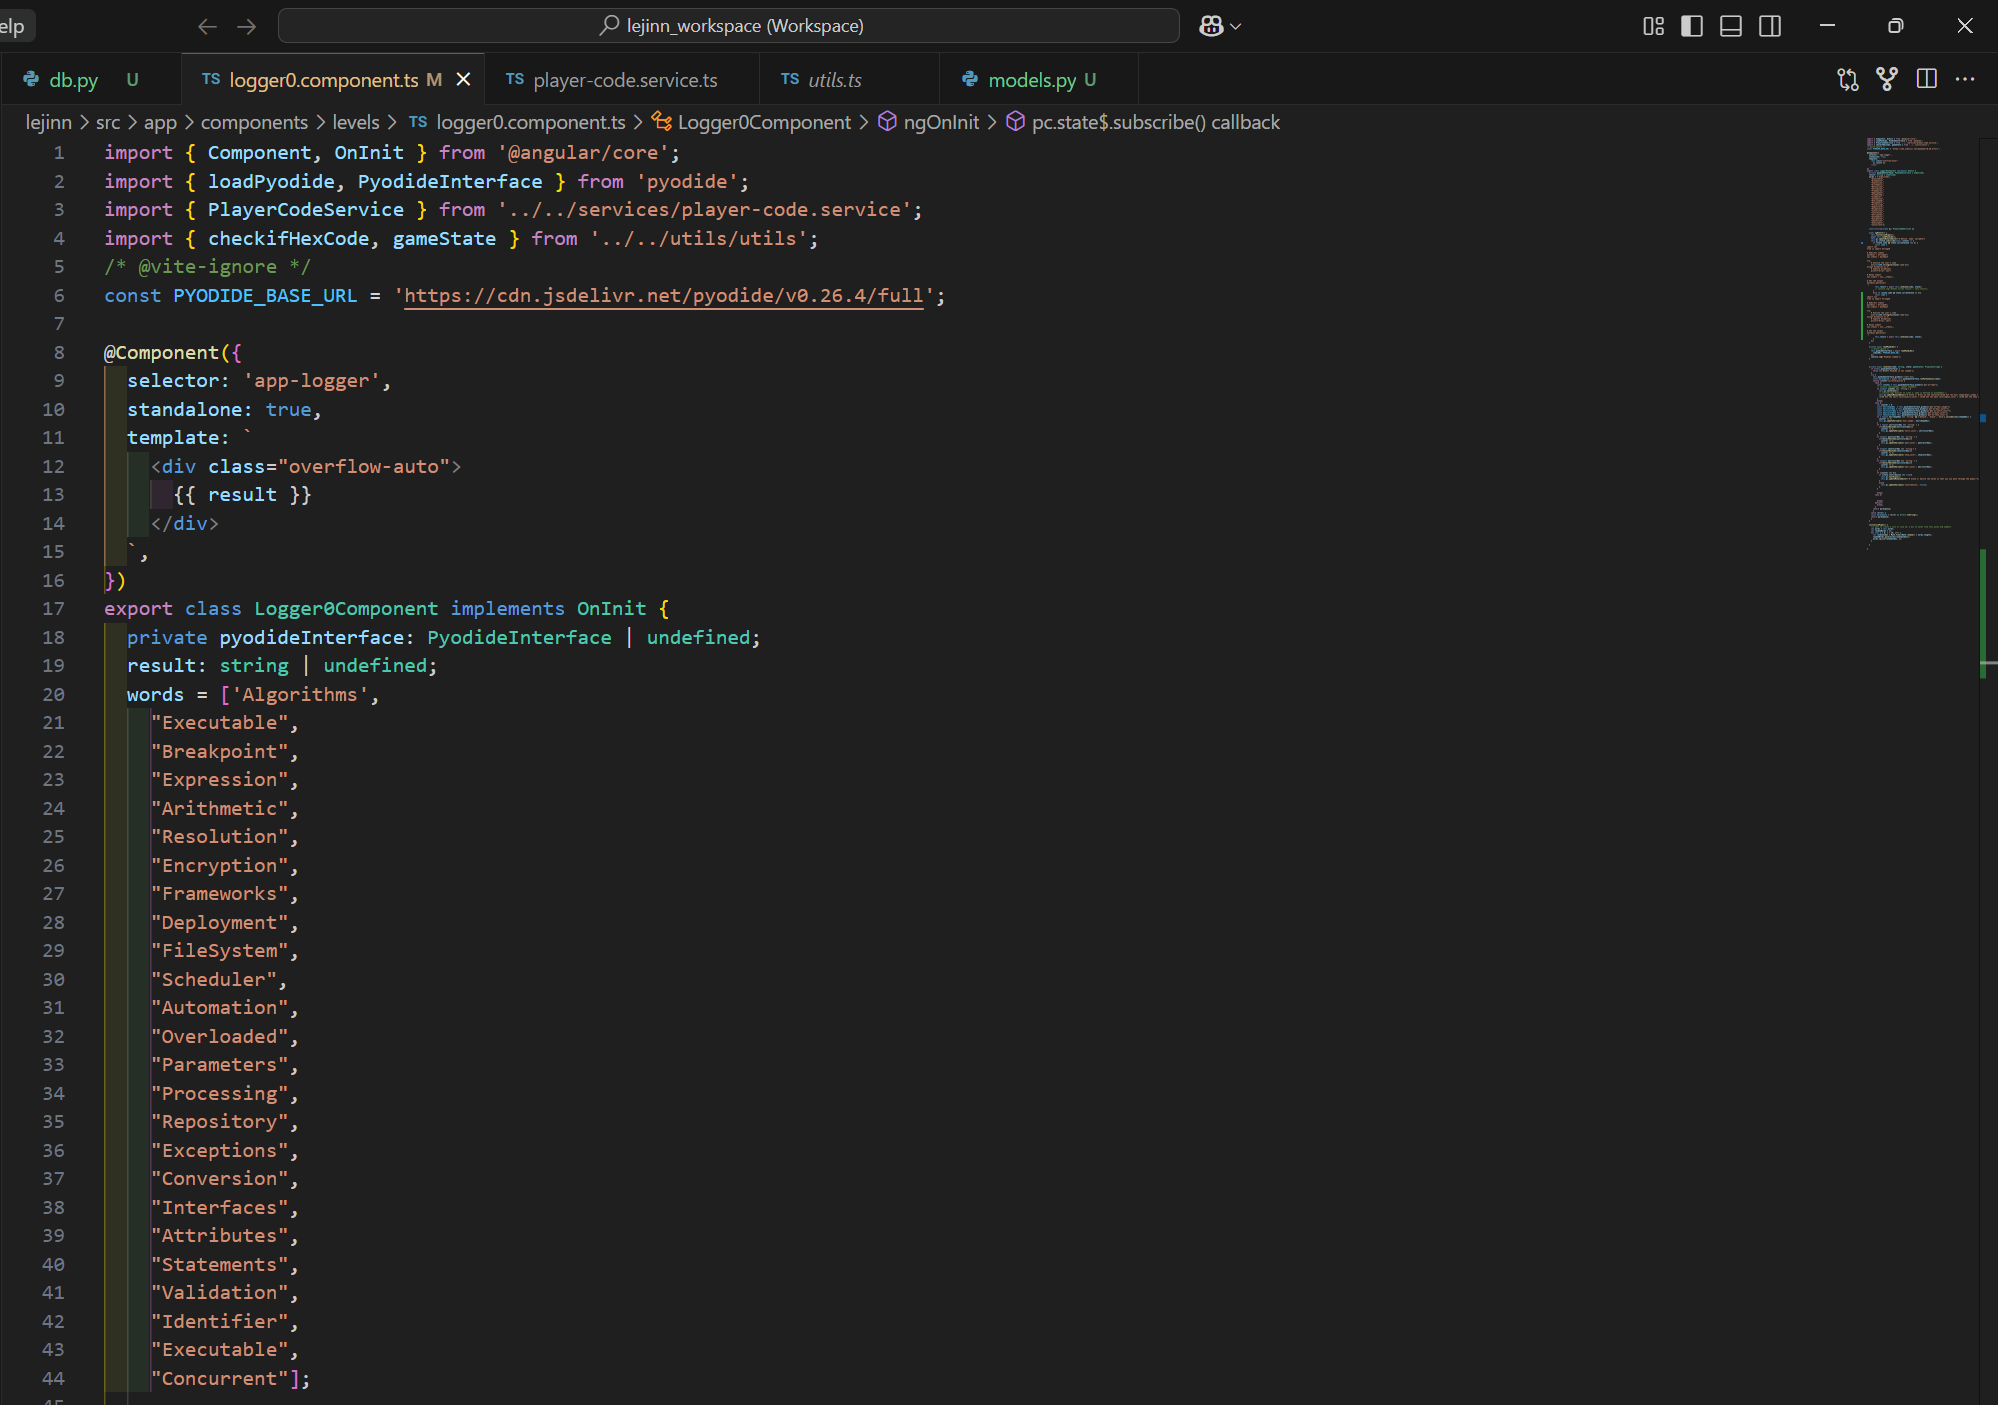
\includegraphics[width=0.3\linewidth]{images/code_editor.png}
    \caption{Code editor of IDE, a significant improvement over a basic textbox}
\end{figure}
Upon code submission, there is a reaction of the code that ran. This reaction of running code is usually known as standard output(stdout). This has to be printed out, including all results and any errors of the code. Other than just text printing with results of code submission, storytelling can take place here that is reactive upon successful results. 
